\documentclass[border=4pt]{standalone}

% --- packages (mirror these in database.meta.json "requires") ---
\usepackage{tikz}

% --- palette (canonical source: reference/color-palettes/color-palettes.md; light variant) ---
\definecolor{otblue}{HTML}{0072B2}
\definecolor{otorange}{HTML}{E69F00}
\definecolor{otteal}{HTML}{009E73}
\definecolor{otpurple}{HTML}{CC79A7}
\definecolor{otgray}{HTML}{5A5A5A}

\begin{document}
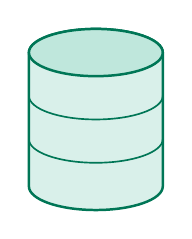
\begin{tikzpicture}[line width=0.9pt]
  \def\rx{0.85}   % x-radius of the cylinder
  \def\ry{0.30}   % y-radius of the top/bottom ellipses
  \def\bh{1.7}    % body height
  % body (sides + bulging bottom, closed over the top)
  \filldraw[draw=otteal!75!black, fill=otteal!15]
    (-\rx,0) -- (-\rx,-\bh)
    arc[start angle=180, end angle=360, x radius=\rx, y radius=\ry]
    -- (\rx,0)
    arc[start angle=0, end angle=180, x radius=\rx, y radius=\ry] -- cycle;
  % top rim
  \filldraw[draw=otteal!75!black, fill=otteal!25] (0,0) ellipse[x radius=\rx, y radius=\ry];
  % stripe bands (front halves)
  \draw[draw=otteal!75!black, line width=0.6pt]
    (-\rx,-0.55) arc[start angle=180, end angle=360, x radius=\rx, y radius=\ry];
  \draw[draw=otteal!75!black, line width=0.6pt]
    (-\rx,-1.10) arc[start angle=180, end angle=360, x radius=\rx, y radius=\ry];
\end{tikzpicture}
\end{document}
